%-----------------------------------LICENSE------------------------------------%
%   This file is part of tikz_figures.                                         %
%                                                                              %
%   tikz_figures is free software: you can redistribute it and/or              %
%   modify it it under the terms of the GNU General Public License as          %
%   published by the Free Software Foundation, either version 3 of the         %
%   License, or (at your option) any later version.                            %
%                                                                              %
%   tikz_figures is distributed in the hope that it will be useful,            %
%   but WITHOUT ANY WARRANTY; without even the implied warranty of             %
%   MERCHANTABILITY or FITNESS FOR A PARTICULAR PURPOSE.  See the              %
%   GNU General Public License for more details.                               %
%                                                                              %
%   You should have received a copy of the GNU General Public License along    %
%   with tikz_figures.  If not, see <https://www.gnu.org/licenses/>.           %
%------------------------------------------------------------------------------%

% Use the standalone class for displaying the tikz image on a small PDF.
\documentclass[crop, tikz]{standalone}

% Import the tikz package to use for the drawing.
\usepackage{tikz}

% tikz libraries used in the drawing.
\usetikzlibrary{
    angles, % Drawing angles within triangles.
    quotes  % Adding labels to angles.
}

% Begin the document.
\begin{document}

    % Draw the figure.
    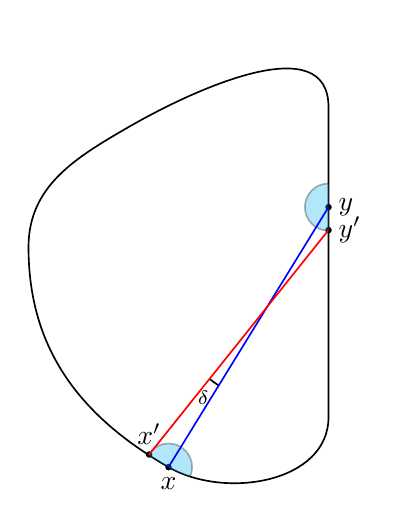
\begin{tikzpicture}[%
        line width = 0.6pt,
        line cap = round
    ]

        % Nodes for the points of interest.
        \coordinate (x) at (-0.3in, -1.0in);
        \coordinate (y) at (0.5in, 0.3in);
        \coordinate (xp) at (-0.397in, -0.937in);
        \coordinate (yp) at (0.5in, 0.185in);
        \coordinate (O) at (0.2in, -0.19in);

        % Add labels for these points.
        \node at (x) [below] {$x$};
        \node at (y) [right] {$y$};
        \node at (xp) [above] {$x'$};
        \node at (yp) [right] {$y'$};

        % More points for the drawing.
        \coordinate (A) at (-1.0in, 0.1in);
        \coordinate (B) at (0.5in,-0.75in);
        \coordinate (C) at (0.5in, 0.8in);
        \coordinate (D) at (-0.5in, 0.7in);

        % Mark the angle delta with a circular arc.
        \pic[%
            draw = black,
            "\scriptsize{${\delta}$}",
            angle eccentricity = 1.2,
            angle radius = 1.2cm
        ] {angle = xp--O--x};

        % Draw in the curve for the convex figure.
        \draw (A) to [out = -90, in = 150]
              (x) to [out = -30, in = -90]
              (B) to [out = 90, in = -90] 
              (C) to [out = 90, in = 30] 
              (D) to [out = -150, in = 90] cycle;

        % Add dots to label the points.
        \draw[fill = black] (x) circle (0.3mm);
        \draw[fill = black] (y) circle (0.3mm);
        \draw[fill = black] (xp) circle (0.3mm);
        \draw[fill = black] (yp) circle (0.3mm);

        % Clip so that the cyan regions below do not fill outside of the figure.
        \clip (A) to [out = -90, in = 150]
              (x) to [out = -30, in = -90]
              (B) to [out = 90, in = -90] 
              (C) to [out = 90, in = 30] 
              (D) to [out = -150, in = 90] cycle;

        % Mark off the two regions of interest with cyan.
        \draw[fill = cyan, opacity = 0.3] (x) circle (3mm);
        \draw[fill = cyan, opacity = 0.3] (y) circle (3mm);

        % Connect the dots.
        \draw[draw = blue] (x) to (y);
        \draw[draw = red] (xp) to (yp);
    \end{tikzpicture}
\end{document}
